
%(BEGIN_QUESTION)
% Copyright 2007, Tony R. Kuphaldt, released under the Creative Commons Attribution License (v 1.0)
% This means you may do almost anything with this work of mine, so long as you give me proper credit

Shown here is a simple feedforward control system (with trim), which attempts to compensate for changes in cold feed flow by immediately adjusting fuel flow to the burners proportionately ({\it before} the outlet temperature has time to change):

$$\includegraphics[width=15.5cm]{i01779x01.eps}$$

\filbreak

A problem lurks within this process, however, which is not very obvious.  The problem is {\it lag time}.  Imagine removing all automatic controls from the process, and replacing them with hand valves so we could have manual control over feed flow and fuel flow while we graphed outlet temperature on a trend recorder:

$$\includegraphics[width=15.5cm]{i01779x02.eps}$$

\filbreak

Now, imagine introducing a step change in feed flow, and a step change in fuel gas flow, in two separate tests:

$$\includegraphics[width=15.5cm]{i01779x03.eps}$$

If these two lag times (one for feed flow and one for fuel flow) are exactly the same, then a simple feedforward compensation system such as that shown at the beginning of the question will work just fine.  However, if these lag times are {\it not} equal, as shown in above trends, a simple feedforward system will not perfectly compensate for changes in feed flow.  Explain why.

\underbar{file i01779}
%(END_QUESTION)





%(BEGIN_ANSWER)

If the two lag times are unequal, the feedforward response to a change in feed flow may either be too soon, or too late.  

\vskip 10pt

Follow-up question: given the lag times shown in the ``manual test'' trends, would the fuel gas adjustment be too soon or too late to compensate for a change in feed rate?

%(END_ANSWER)





%(BEGIN_NOTES)

In the manual test shown, the fuel flow lag time is shorter than the feed flow lag time.  This means the feedforward compensation will come {\it too soon}.

%INDEX% Control, strategies: feedforward (analysis of lag times)
%INDEX% Process: heater (fired) (generic)

%(END_NOTES)


